\documentclass[conference]{IEEEtran}
\usepackage{graphicx}
\usepackage{lipsum} % solo para generar texto de ejemplo
\usepackage[english]{babel}
%Includes "References" in the table of contents
\usepackage[nottoc]{tocbibind}

\begin{document}

\title{Análisis, visualización y predicción de Precios Airbnb}

\author{%
\IEEEauthorblockN{Martín Navarrete Villegas}
\IEEEauthorblockA{Facultad De Ciencias Fisicomatemáticas\\
Universidad Autónoma de Nuevo León\\
Correo electrónico: martin.nv6@gmail.com\\}
}

\maketitle

\begin{abstract}
  El objetivo de este documento es desarrollar un modelo confiable de predicción de precios para propiedades de alquiler en Airbnb utilizando técnicas de aprendizaje automático. Se utilizarán características de alquileres y reseñas de clientes como predictores y se aplicarán una variedad de métodos, incluyendo regresión lineal, modelos basados en árboles, regresión Ridge, Lasso y Random Forest, para crear el modelo de predicción. El objetivo final es ayudar a propietarios y clientes a evaluar el precio óptimo de una propiedad con información limitada disponible.
\end{abstract}

% Keywords command
\providecommand{\keywords}[1]
{
  \small	
  \textbf{\textit{Palabras clave---}} #1
}
\keywords{airbnb, predicción, precio, nueva york, regresión.}

\section{Introducción}
La era de la pandemia de covid nos obligo a cambiar nuestra forma de vivir, con ello la manera en la que viajamos y nos hospedamos cambio, Airbnb es un servicio de interenet que provee la plataforma para conectar propietarios de casas o departamentos con clientes potenciales, durante la pandemia esta plataforma alcanzo niveles de uso muy altos, se realizo una comparación de exactitud de modelos de regresión para predicción de precios de hospedajes en Airbnb basado en una serie de parámetros como el tipo de habitación, la cantidad de opiniones en el sitio, cantidad de días de ocupación y el barrio.

\subsection{Objetivo principal}
Realizar una comparación de exactitud de modelos de regresión para predicción de precios de hospedajes en Airbnb.
\subsection{Objetivo secundario}
 Con los resultados lograr encontrar un algoritmo de predicción de precios que pueda ser utilizado para calcular precios y encontrar las variables mas determinantes.

\section{Antecedentes}
Partes de la literatura existente sobre precios de propiedades se enfocan en la compra de propiedades no compartidas o predicciones de precios de alquiler. Previamente, Yu y Wu [1] intentaron implementar una predicción de precios de bienes raíces utilizando un análisis de importancia de características junto con regresión lineal, SVR y regresión Random Forest. También intentaron clasificar los precios en 7 clases utilizando Naive Bayes, Logistic Regression, SVC y Random Forest. Declararon un mejor RMSE de 0,53 para su modelo SVR y una precisión de clasificación del 69\% para su modelo SVC con PCA. En otro artículo, Ma et al. [2] han aplicado Regresión Lineal, Árbol de Regresión, Regresión de Bosque Aleatorio y Árboles de Regresión de Aumento de Gradiente para analizar los precios de alquiler de almacenes en Beijing. Llegaron a la conclusión de que el modelo de regresión de árbol fue el modelo de mejor rendimiento con un RMSE de 1,05 CNY/m2-día. Otra clase de estudios, que son más pertinentes para este trabajo, inspeccionan los hoteles y los precios de alquiler de la economía compartida. En un trabajo reciente, Wang y Nicolau [3] estudiaron los determinantes de los precios de la economía colaborativa mediante el análisis de listados de Airbnb utilizando mínimos cuadrados ordinarios y análisis de regresión por cuantiles.

\section{Descripción de datos}
El conjunto de datos públicos de Airbnb para la ciudad de Nueva York se utilizó como fuente de datos principal para este estudio. El conjunto de datos incluía 50.221 entradas, cada una con 96 funciones. La figura 1 muestra la distribución geográfica de los precios de cotización en este conjunto de datos.
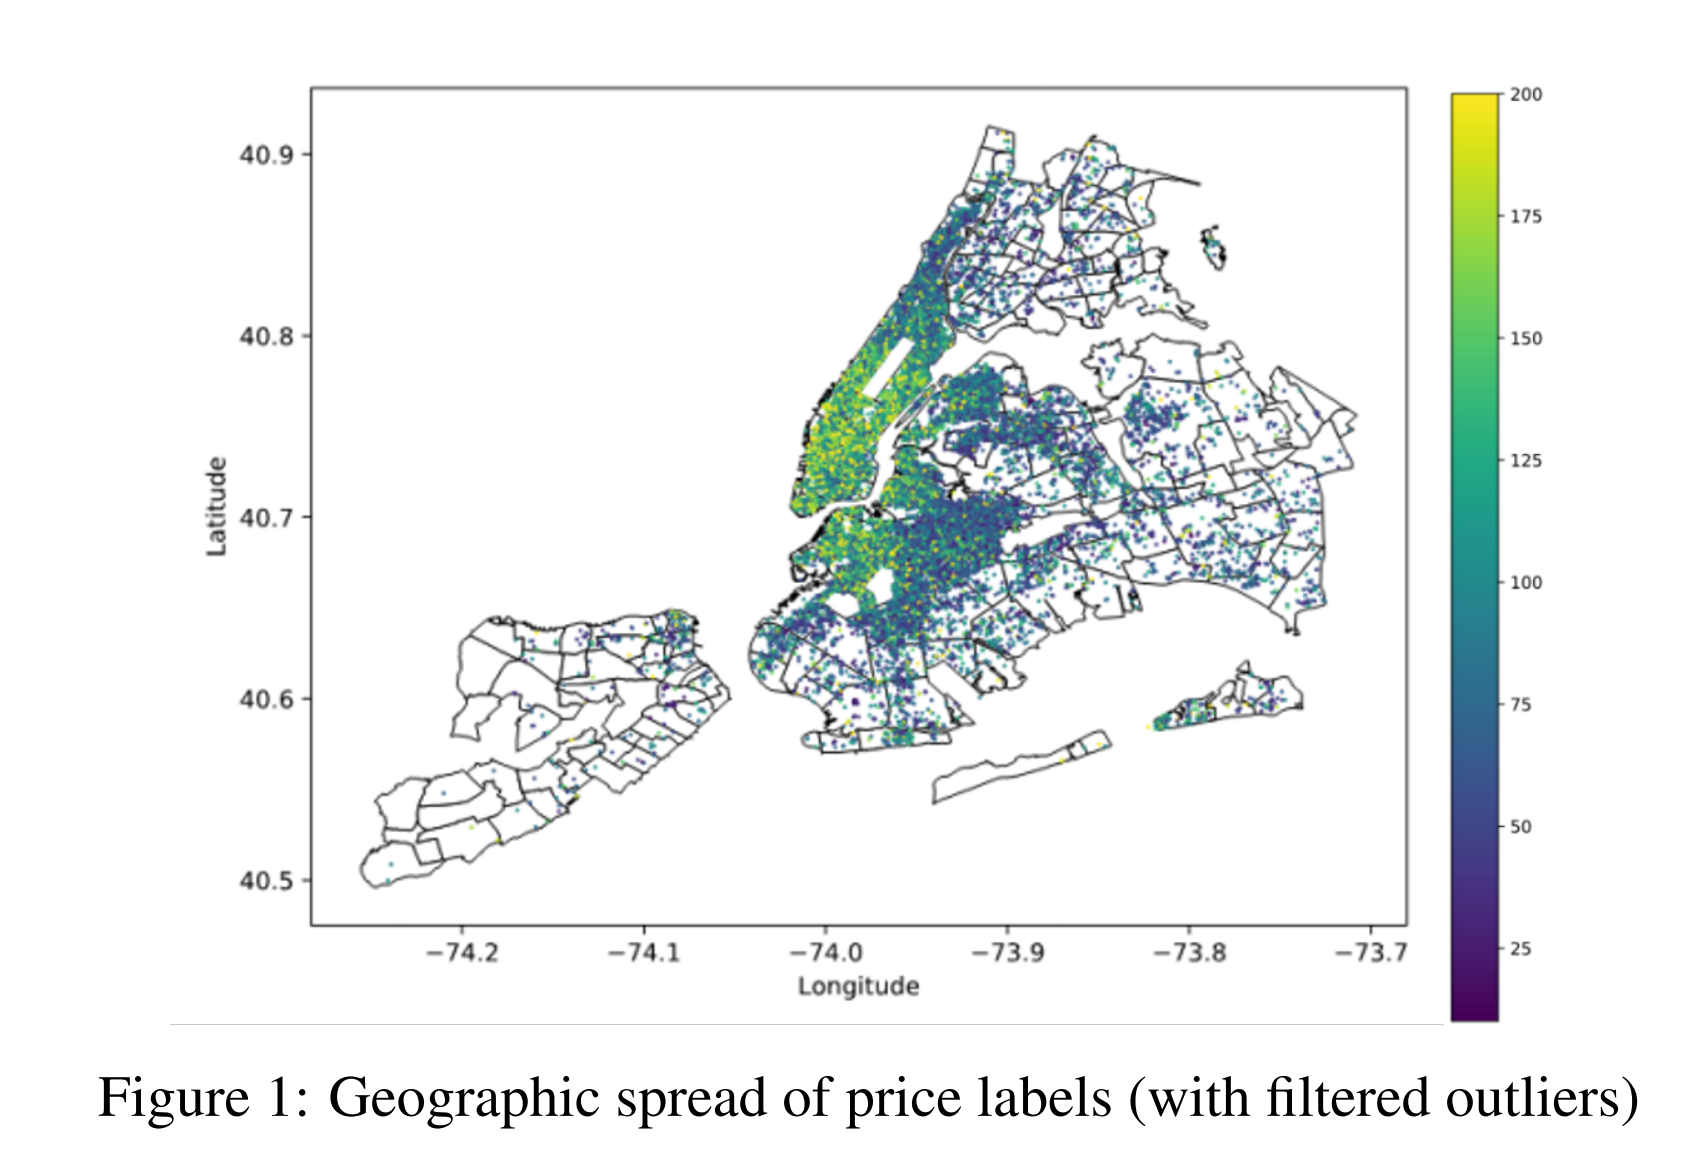
\includegraphics[width=10cm]{images/figura1.png}

\section{Metodología}
En el siguiente diagrama se muestra la metodología que se siguió para esta investigación
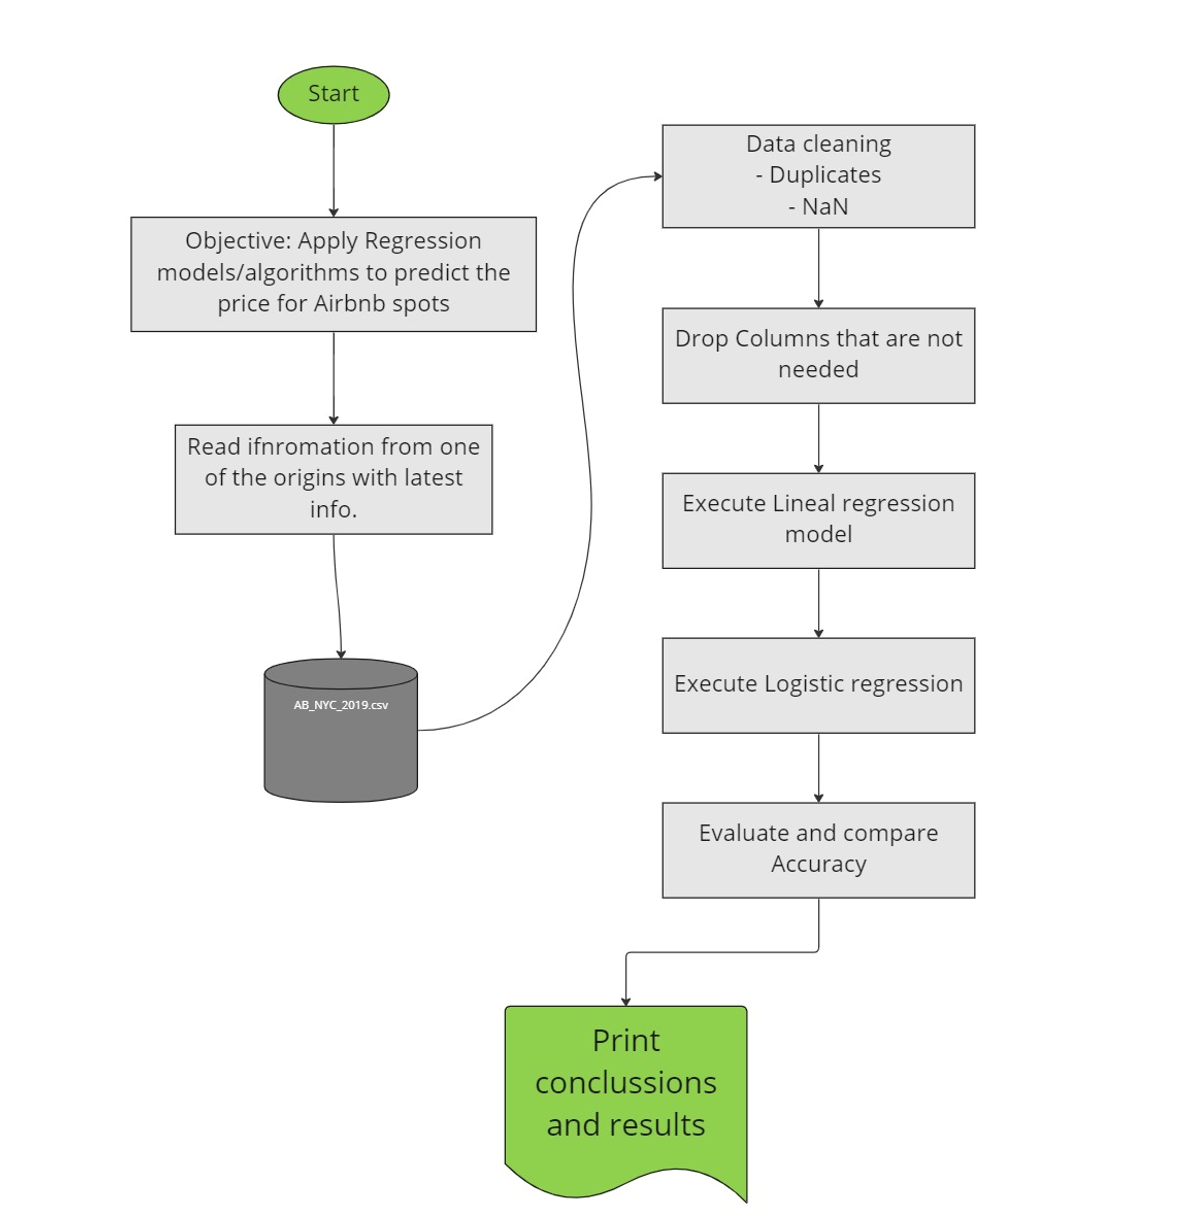
\includegraphics[width=10cm]{images/Metodologia.png}

Se comienza con lectura de los datos y con limpieza de estos, para ello se hace lo siguiente 
\begin{enumerate}
    \item Remover duplicados
    \item Encontrar los valores nulos
    \item Reparar los valores nulos 
    \item En el caso de los valores nulos de 'reviewsPerMonth' se realiza un cambio de nulos por cero
    \item Algunos campos son eliminados como el name, id, host name, last review, reviews per month, calculated host listings count
    \item Se limpian los outliers [Figura2]
    \item Se generan dummies para conversión de features categóricas a ficticias [Figura3]
    \item Regresión lineal
      \begin{enumerate}
        \item La regresión lineal que utiliza todo el conjunto de características como entradas del modelo se tomó como modelo de referencia para
        evaluando el desempeño de los otros métodos.
      \end{enumerate}
    \item Regresión Ridge
      \begin{enumerate}
        \item La regresión lineal con regularización L2 agrega un término de penalización a la función de costo del error cuadrático en
        para ayudar al algoritmo a converger para datos linealmente separables y reducir el sobre ajuste.
        \item Dado que se observó que los modelos de referencia tenían una varianza alta, Ridge Regression parecía ser una opción adecuada para resolver el problema.
      \end{enumerate}
    \item Regresión Laso
      \begin{enumerate}
        \item Tomando como consideración los resultados obtenidos en Regresion Ridge y lineal se decidió continuar con la ejecución de los siguientes modelos, con la intención de realizar suficientes comparaciones de resultados.
      \end{enumerate}
    \item Regresión de Árbol de Decisión
      \begin{enumerate}
        \item A pesar que se preveía que no seria un modelo útil se ejecuto par fines comparativos
      \end{enumerate}
    \item Regresión Random Forest
      \begin{enumerate}
        \item A pesar que se preveía que no seria un modelo útil se ejecuto par fines comparativos
      \end{enumerate}
\end{enumerate}

\section{Resultados}
Como parte de los resultados de la eliminación de outlieres concluimos con lo que muestra la siguiente figura [figura2]
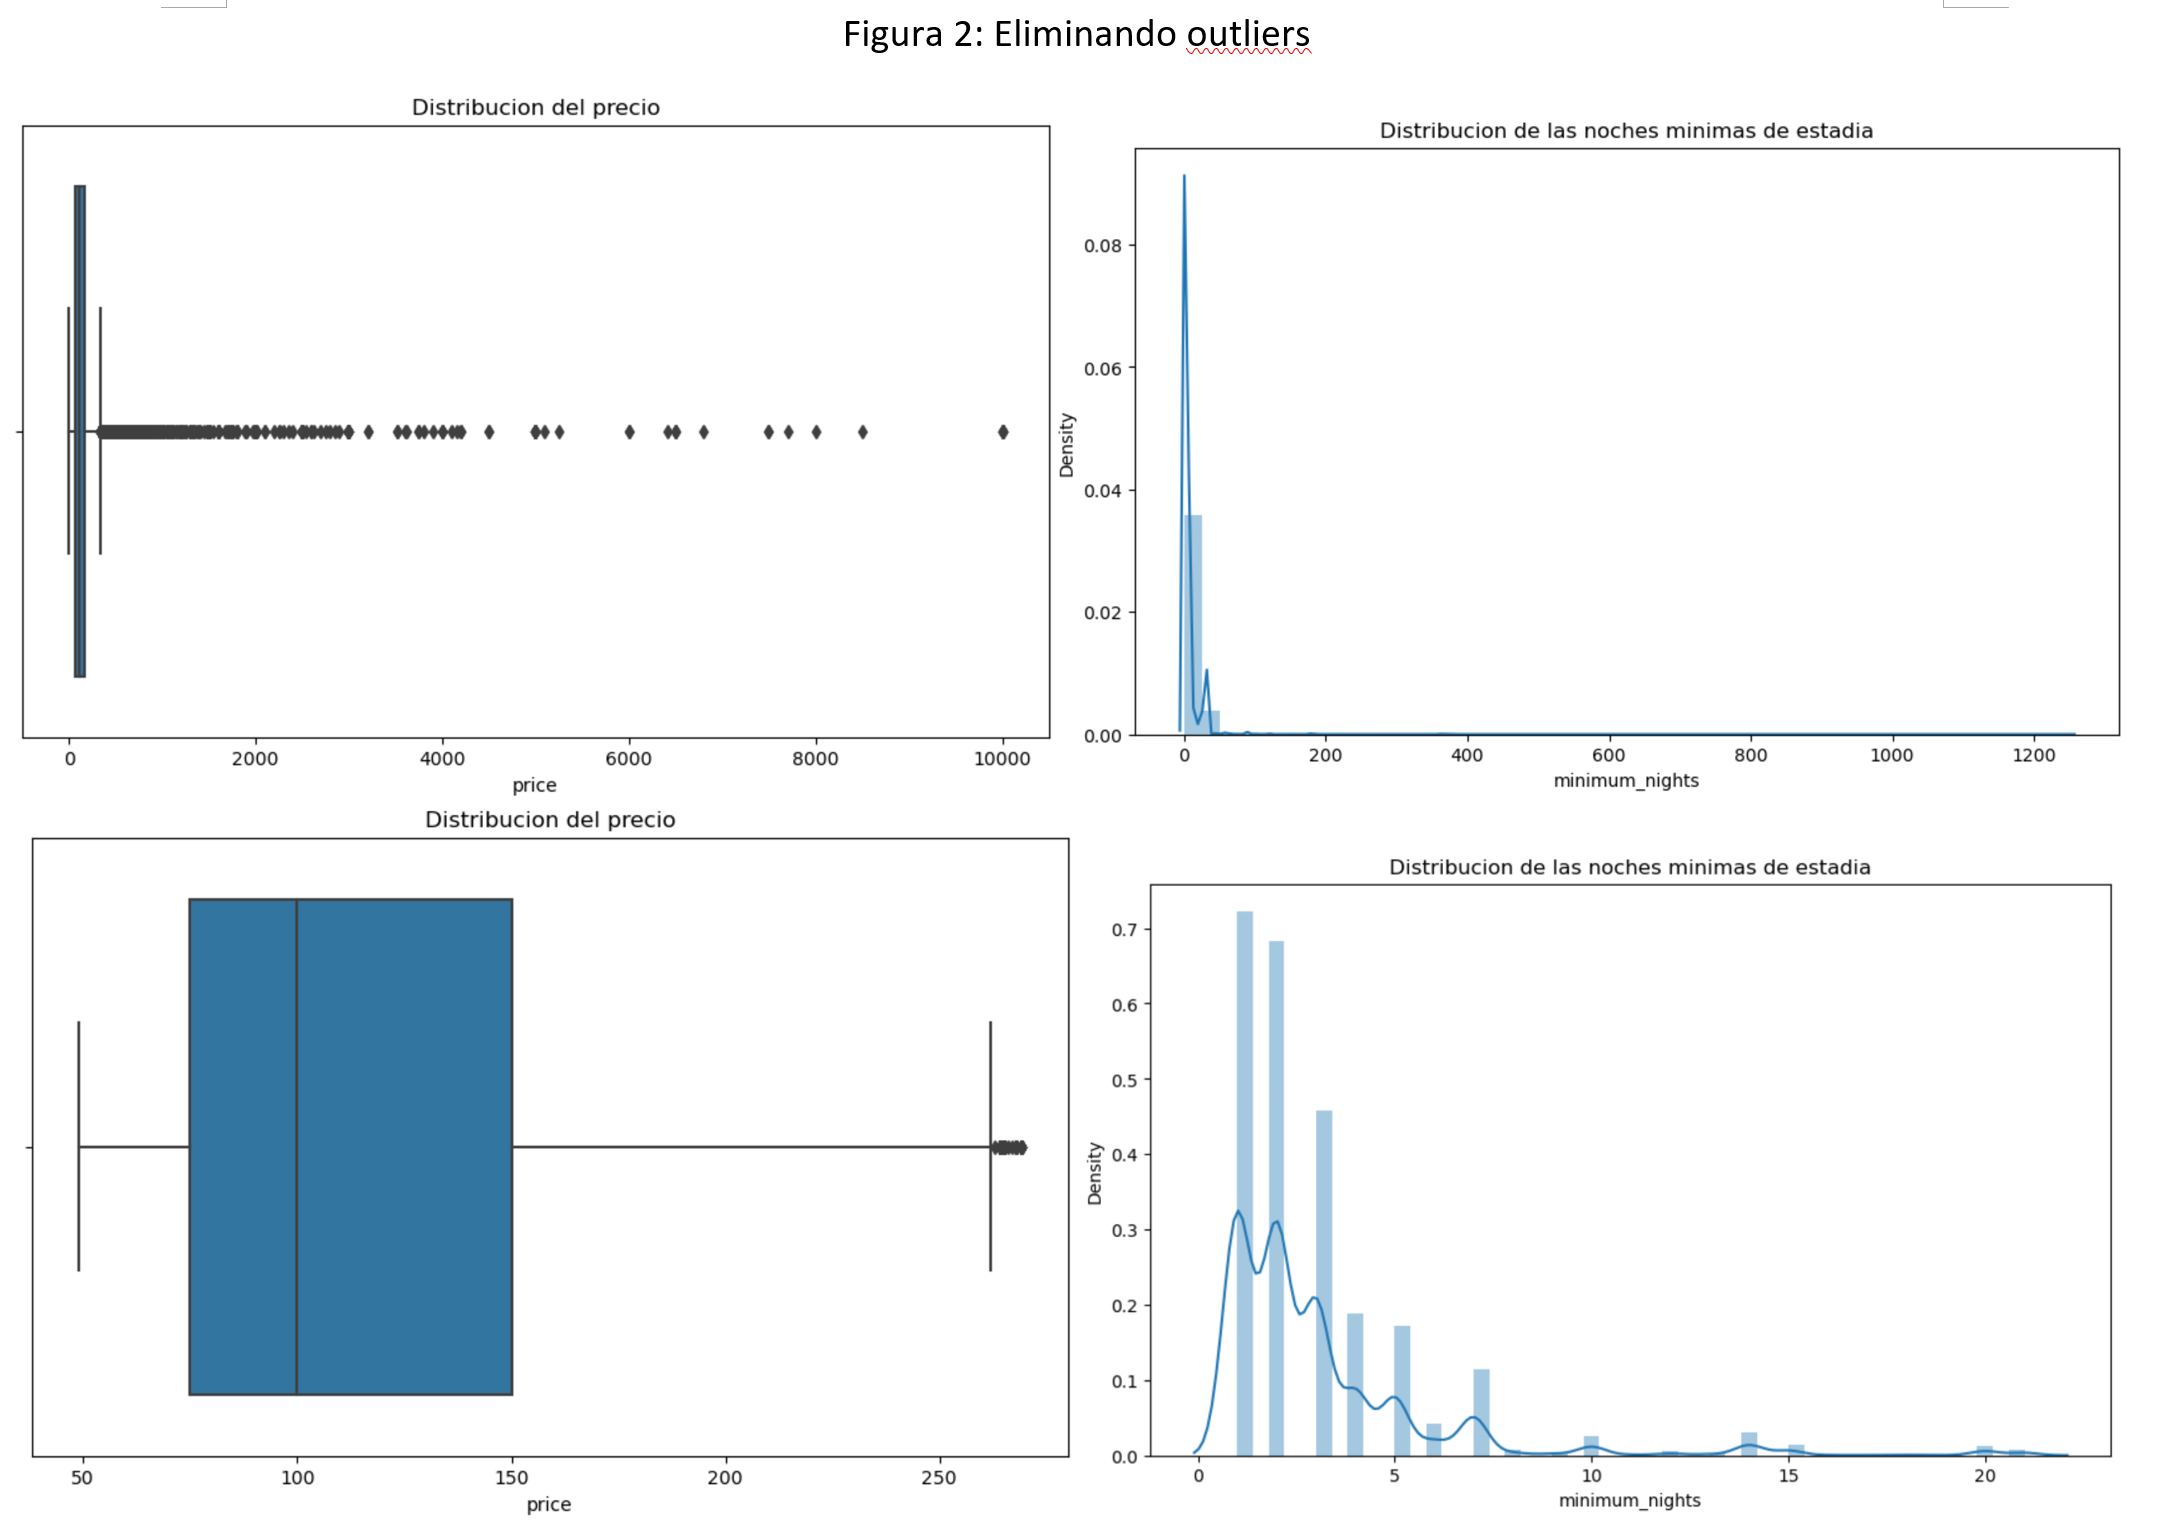
\includegraphics[width=10cm]{images/figura2.png}

Los dummies generados se muestran en la siguiente figura [figura3]
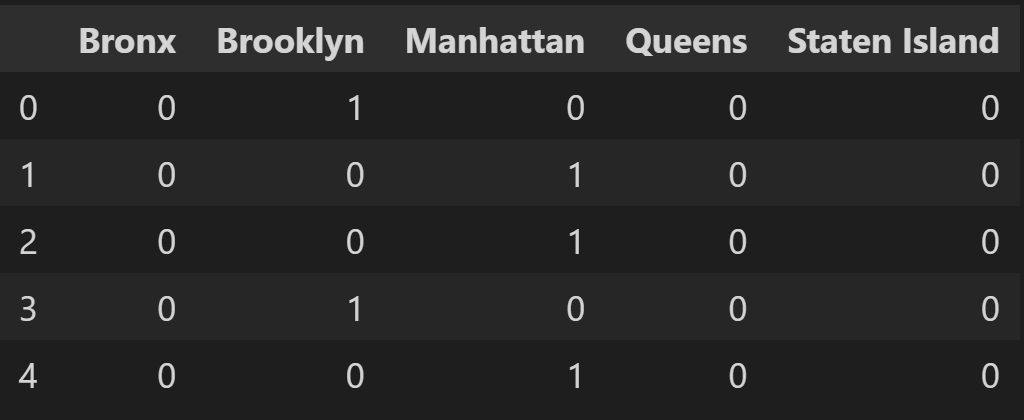
\includegraphics[width=10cm]{images/figura3.png}

En la [tabla 1] se muestran las métricas de rendimiento y desempeño de los modelos
Desviación cuadrática media (RMSE) y R2
sirvieron para evaluar la
modelos entrenados.
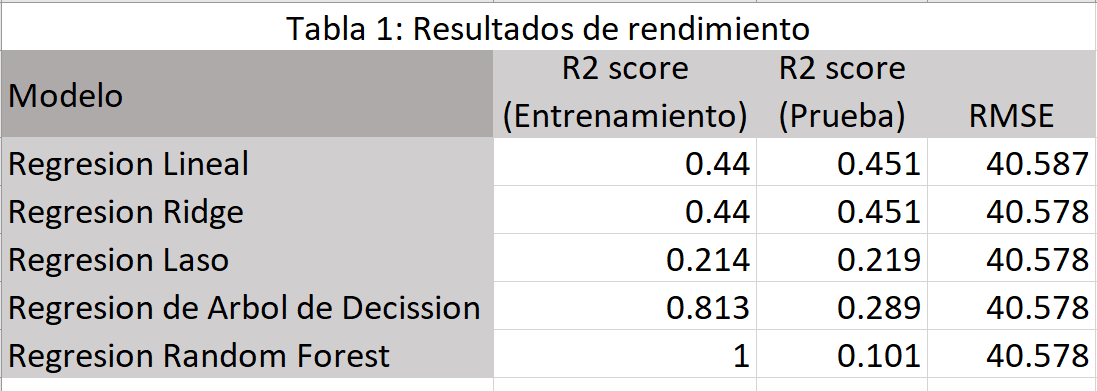
\includegraphics[width=10cm]{images/tabla1.png}

\section{Conclusiones}
Regresión Ridge y Regresión lineal tenían R2 similar y 
aunque el último modelo es más complejos que la regresión lineal. Se cree que la complejidad de la arquitectura
de una red neuronal estaría limitada por la cantidad insuficiente de ejemplos de entrenamiento por tener demasiados
pesos desconocidos.

Los datos indican que la Regresión de Laso no cuenta con puntuación suficiente como para ser considerado un modelo óptimo.
Los resultados para Random forest y arbol de decisiones son muy ambiguos y no nos indican si el modelo es óptimo, además que el error de desviación cuadrática (RMSE) es alto llegando a 40.578\% como se muestra en [tabla1]

\section{Trabajo a futuro}
Debido a que los resultados no fueron del todo satisfactorios en términos de precisión por encima del 50\%, como trabajo a futuro se realizara el procedimiento pero usando algoritmos de clasificación, de esta manera quizá se logre un mejor resultados buscando precios "bajos", "medios" y "altos".
\vspace{5mm} %5mm vertical space

\bibliographystyle{ieeetr}
\bibliography{referencias} % aquí debes reemplazar "referencias" con el nombre de tu archivo .bib que contenga las referencias
\cite{Hyu2016,DWang2018,Schwarzova_undated-cm,Schwarzova2020-ud,Kalehbasti2020-sk}
\end{document}